\section{Мета роботи}
Набуття і закріплення навичок програмування розміщення в пам’яті специфічних масивів.

\section{Хід роботи}
    Розробити спосіб економного розміщення в пам’яті заданої
розрідженої таблиці, де записані цілі числа. Розробити функції, що
забезпечують доступ до елементів таблиці за номерами рядка і стовпця.\\

    У програмі забезпечити запис і читання всіх елементів таблиці.\\

    Визначити та порівняти час доступу до елементів таблиці при
традиційному та економному поданні її в пам’яті. Зробити висновки.\\

    Завдання обрати з табл. 5.1 згідно із своїм номером у журналі групи.\\

    \textbf{Моє завдання:} нульові елементи розташовані на місцях з парними індексами
    рядків і стовпців.


\subsection{Обраний підхід до побудови таблиці}
Для вирішення моєї задачі я вирішив використовувати формат розріджених рядків (\textbf{CSR — Compressed Sparse Row}). Після досілдження інформації, я зрозумів що цей метод є ефективним для зберігання розрідженних таблиць та забезпечує оптимальний доступ до них по рядкам та стовбцях. \\

    Формат CSR зберігає ненульові елементи з їхніми відповідними індексами стовпців і 
покажчиками на початок кожного рядка, що робить його особливо зручним для випадків, де 
нульові елементи мають специфічний розподіл.

\clearpage
\subsection{Реалізація CSR таблиці}

    В приведеній нижче реалізації було створено міні-бібліотеку для переведення
звичайної матриці у CSR формат та також додаткові методи для роботи з ними.\\

    Було реалізовано такі методи: \textbf{створення таблиці, отримання елемента за індексом, 
    вивід таблиці, знищення таблиці.}

\begin{lstlisting}[style=customc]
#include <stdio.h>
#include <stdlib.h>

typedef struct {
  int *values;
  int *colIndex;
  int *rowPtr;
  int nonZeroCount;
} CSRMatrix;

CSRMatrix create(int **matrix, int rows, int cols) {
  CSRMatrix csr;
  int nonzero_elem_count = 0;

  for (size_t i = 0; i < rows; i++) {
    for (size_t j = 0; j < cols; j++) {
      if (!(i % 2 == 0 && j % 2 == 0) && matrix[i][j] != 0) {
        nonzero_elem_count++;
      }
    }
  }

  csr.values = (int *)malloc(nonzero_elem_count * sizeof(int));
  csr.colIndex = (int *)malloc(nonzero_elem_count * sizeof(int));
  csr.rowPtr = (int *)malloc((rows + 1) * sizeof(int));
  csr.nonZeroCount = nonzero_elem_count;

  int k = 0;
  csr.rowPtr[0] = 0; // start of first row
  for (size_t i = 0; i < rows; i++) {
    for (size_t j = 0; j < cols; j++) {
      if (!(i % 2 == 0 && j % 2 == 0) && matrix[i][j] != 0) {
        csr.values[k] = matrix[i][j];
        csr.colIndex[k] = j;
        k++;
      }
    }
    csr.rowPtr[i + 1] = k; // end of current row
  }

  return csr;
}

int get_element(CSRMatrix *csr, int row, int col) {
  for (size_t i = csr->rowPtr[row]; i < csr->rowPtr[row + 1]; i++) {
    if (csr->colIndex[i] == col) {
      return csr->values[i];
    }
  }

  return (row % 2 == 0 && col % 2 == 0) ? 0 : 0;
}

void print(CSRMatrix csr, int rows, int cols) {
  printf("\033[33mValues:\033[0m ");
  for (int i = 0; i < csr.nonZeroCount; i++) {
    printf("%d ", csr.values[i]);
  }
  printf("\n\033[33mColumn indexes for non-zero elements:\033[0m ");
  for (int i = 0; i < csr.nonZeroCount; i++) {
    printf("%d ", csr.colIndex[i]);
  }
  printf("\n\033[33mPointers to the beginning of each row in the values "
         "array:\033[0m ");
  for (int i = 0; i <= rows; i++) {
    printf("%d ", csr.rowPtr[i]);
  }
  printf("\n");
}

void destroy(CSRMatrix *csr) {

  if (csr->values != NULL) {
    free(csr->values);
    csr->values = NULL;
  }
  if (csr->colIndex != NULL) {
    free(csr->colIndex);
    csr->colIndex = NULL;
  }
  if (csr->rowPtr != NULL) {
    free(csr->rowPtr);
    csr->rowPtr = NULL;
  }
  csr->nonZeroCount = 0;
}

\end{lstlisting}

\clearpage
\subsection{Реалізація звичайної матриці}
    Для порівняння роботи CSR матриці зі звичайною, я окремо розробив методи
для роботи зі звичайною матрицею.\\

    Було створено такі методи: \textbf{вивід матриці, заповнення випадковими цілими числами, 
знищення матриці.}

\begin{lstlisting}[style=customc]
void print_matrix(int **matrix, int rows, int cols) {
  for (int i = 0; i < rows; i++) {
    for (int j = 0; j < cols; j++) {
      if (matrix[i][j] == 0) {
        printf("\033[33m%d\033[0m ", matrix[i][j]);
      } else {
        printf("%d ", matrix[i][j]);
      }
    }
    printf("\n");
  }
}

void free_matrix(int **matrix) {
  for (int i = 0; i < N; i++) {
    free(matrix[i]);
  }
  free(matrix);
}

void fill_matrix(int **matrix) {
  for (int i = 0; i < N; i++) {
    matrix[i] = (int *)malloc(N * sizeof(int));
    for (int j = 0; j < N; j++) {
      matrix[i][j] = generateRandomInt(10, 80);
      if (i % 2 == 0 && j % 2 == 0) {
        matrix[i][j] = 0;
      }
    }
  }
}

\end{lstlisting}

\clearpage
\subsection{Реалізація основної програми}
    Тут було реалізовано основну програму з використанням звичайної матриці та її
парсингом у CSR матрицю. Було порівняно доступ до елементів та вивід представлення 
матриць у консоль.

\begin{lstlisting}[style=customc]
#include <stdio.h>
#include <stdlib.h>

#include "general_utils.h"
#include "sparse_table.h"

#define N 5

void print_matrix(int **matrix, int rows, int cols) {
  for (int i = 0; i < rows; i++) {
    for (int j = 0; j < cols; j++) {
      if (matrix[i][j] == 0) {
        printf("\033[33m%d\033[0m ", matrix[i][j]);
      } else {
        printf("%d ", matrix[i][j]);
      }
    }
    printf("\n");
  }
}

void free_matrix(int **matrix) {
  for (int i = 0; i < N; i++) {
    free(matrix[i]);
  }
  free(matrix);
}

void fill_matrix(int **matrix) {
  for (int i = 0; i < N; i++) {
    matrix[i] = (int *)malloc(N * sizeof(int));
    for (int j = 0; j < N; j++) {
      matrix[i][j] = generateRandomInt(10, 80);
      if (i % 2 == 0 && j % 2 == 0) {
        matrix[i][j] = 0;
      }
    }
  }
}

void task1() {
  int **matrix = (int **)malloc(N * sizeof(int *));
  clock_t start_time, end_time;
  double access_time;

  highlightText("ORIGINAL MATRIX", "blue");

  printf("\n");
  fill_matrix(matrix);
  print_matrix(matrix, N, N);
  printf("\n");

  start_time = clock();
  printf("Access element at \033[33m(3, 1)\033[0m: %d\n", matrix[3][1]);
  printf("Access element at \033[33m(0, 0)\033[0m: %d\n", matrix[0][0]);
  end_time = clock();
  access_time = ((double)(end_time - start_time)) / CLOCKS_PER_SEC;
  printf("\nTime taken to access elements of matrix: \033[32m%f\033[0m ms\n",
         access_time);
  printf("\n\n\n\n");

  highlightText("ORIGINAL MATRIX CONVERTED TO SPARSE MATRIX", "blue");
  printf("\n");

  CSRMatrix csr = create(matrix, N, N);
  print(csr, N, N);
  printf("\n");

  start_time = clock();
  printf("Access element at \033[33m(3, 1)\033[0m: %d\n",
         get_element(&csr, 3, 1));
  printf("Access element at \033[33m(0, 0)\033[0m: %d\n",
         get_element(&csr, 0, 0));
  end_time = clock();
  access_time = ((double)(end_time - start_time)) / CLOCKS_PER_SEC;
  printf(
      "\nTime taken to access elements of CSR matrix: \033[32m%f\033[0m ms\n",
      access_time);

  free_matrix(matrix);
  destroy(&csr);
}
\end{lstlisting}

\begin{figure}[h!]
    \centering
    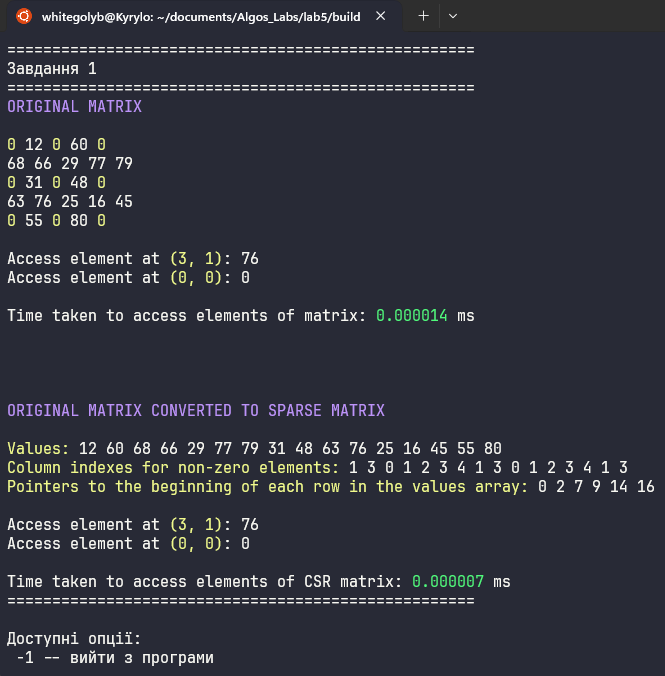
\includegraphics[width=12cm]{reports/algos/lab5/assets/1.png}
    \caption{Результат роботи програми}
\end{figure}

\begin{figure}[h!]
    \centering
    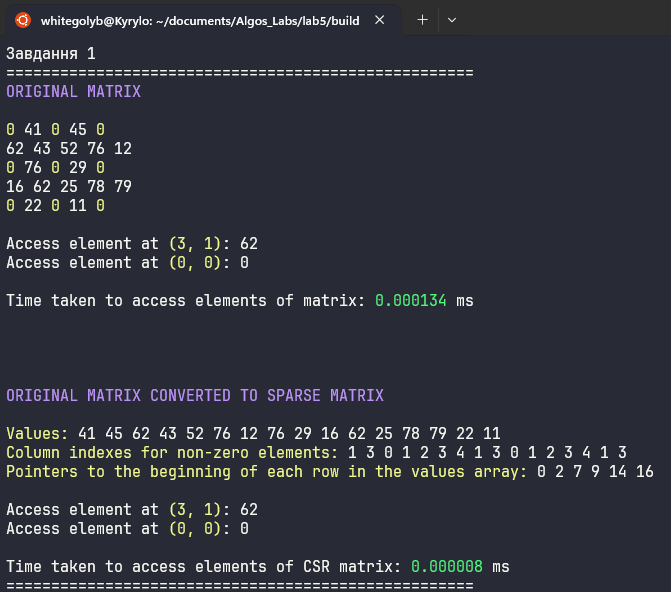
\includegraphics[width=12cm]{reports/algos/lab5/assets/2.png}
    \caption{Результат роботи програми}
\end{figure}

\begin{figure}[h!]
    \centering
    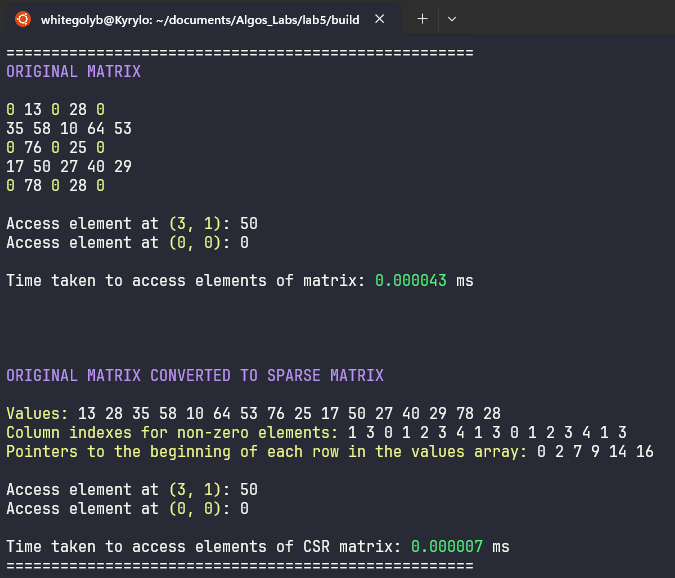
\includegraphics[width=18cm]{reports/algos/lab5/assets/3.png}
    \caption{Результат роботи програми}
\end{figure}

\clearpage
\section{Висновки}
Під час виконання лабораторної роботи, я розібрався з 
розрідженним представленням матриці та розібрався як її
реалізувати для свого завдання. \\

    Проаналізувавши отримані результати після завершення роботи
програми, можна сказати що доступ до елементів звичайної матриці проходить довше ніж до розрідженної, але при певних умовах це може змінитися, бо доступ до елементів звичайної матриці буде швидкішим при більш великих матрицях, бо до елементів можна звертатися через арифметику вказівників, бо матриця зберігається неперервно у пам`яті пристрою. \\

Таким чином можна зробити підсумок:

\begin{itemize}
    \item Якщо матриця майже повністю заповнена ненульовими елементами, \textbf{звичайна матриця} краща для швидкого доступу.
    \item \textbf{Розріджена матриця} виграє, якщо більшість елементів дорівнюють нулю і потрібні операції з усіма ненульовими значеннями, а не точковий доступ до елементів.
\end{itemize}
